% *********************************************************************
% © 2026 Jeremy Sylvestre
%
% Permission is granted to copy, distribute and/or modify this document
% under the terms of the GNU Free Documentation License, Version 1.3 or
% any later version published by the Free Software Foundation; with no
% Invariant Sections, no Front-Cover Texts, and no Back-Cover Texts. A
% copy of the license is included in the appendix entitled “GNU Free
% Documentation License” that appears in the output document of this
% PreTeXt source code. All trademarks™ are the registered® marks of
% their respective owners.
%
% *********************************************************************
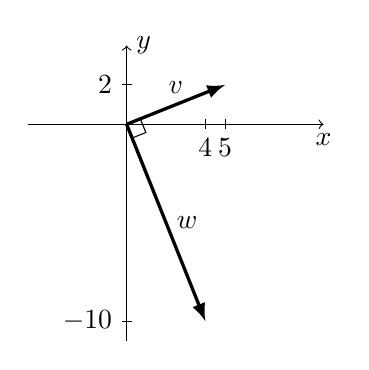
\begin{tikzpicture}[
	vector/.style={-latex,very thick},
	scale=0.25
]
	\draw[->] (-5,0) to (10,0) node[below] {$x$};
	\draw[->] (0,-11) to (0,4) node[right] {$y$};

	\draw[vector] (0,0) to node[above] {$\uvec{v}$} (5,2);
	\draw[thin] (5,0.25) to (5,-0.25) node[below] {$5$};
	\draw[thin] (0.25,2) to (-0.25,2) node[left] {$2$};

	\draw[vector] (0,0) to node[right] {$\uvec{w}$} (4,-10);
	\draw[thin] (4,0.25) to (4,-0.25) node[below] {$4$};
	\draw[thin] (0.25,-10) to (-0.25,-10) node[left] {$-10$};

	% perp symbol
	\draw[thin,rotate=-68.199] (0.75,0) to (0.75,0.75) to (0,0.75);

\end{tikzpicture}
